\documentclass[12pt,a4paper]{article}
\usepackage[utf8]{inputenc}

% Bibliography management
\usepackage[
backend=biber
% citestyle=authoryear,
% style=alphabetic,
% sorting=ynt
]{biblatex}
\addbibresource{bibliography.bib}
% \usepackage[nottoc]{tocbibind}

% Code Listings
\usepackage{listings}
\usepackage{listings-golang} % import this package after listings
\usepackage{color}

% Images
% \usepackage{graphicx}
% \graphicspath{ {images/} }

% Diagrams
\usepackage{tikz}
\usetikzlibrary{shapes, arrows, arrows.meta}

\setlength{\abovecaptionskip}{5px}

\title{A compositional toolkit for the construction of concurrent Web servers}
\author{Michal Bock}
\date{}

\lstset{ % add your own preferences
    frame=single,
    basicstyle=\footnotesize,
    keywordstyle=\color{blue}\bfseries,
    numbers=none,
    showstringspaces=false, 
    stringstyle=\color{red},
    tabsize=4,
    language=Golang,
    belowskip=0px,
    emph={go},
    emphstyle={\color{blue}\bfseries}
}

% Define block styles
\tikzstyle{listener} = [rectangle, draw, fill=gray!60, 
    text width=5em, text centered, minimum height=4em]
\tikzstyle{component} = [rectangle, draw, fill=white, 
    text width=5em, text centered, minimum height=4em]
\tikzstyle{writer} = [rectangle, draw, fill=gray!30, 
    text width=5em, text centered, minimum height=4em]
\tikzstyle{line} = [draw, -latex]

\usepackage[parfill]{parskip}
\usepackage[labelfont=bf]{caption}
\usepackage{hyperref}

\begin{document}

%%%%%%%%%%%%%%%%%%%%%%%%%%%%% Title page %%%%%%%%%%%%%%%%%%%%%%%%%%%%%%
\maketitle
\thispagestyle{empty}

%%%%%%%%%%%%%%%%%%%%%%%%%%%%% Abstract %%%%%%%%%%%%%%%%%%%%%%%%%%%%%%%%

\newpage
\section*{Abstract}
\begin{quote}
The goal of this project is to construct a well-structured
library of communicating components, in the Go language, to support
the programming of a family of webservers that could range in scale 
from a full-scale commercial server to an embedded server used to provide 
a browser-based GUI to a specific application.
\end{quote}

%%%%%%%%%%%%%%%%%%%%%%%%%%%%% Contents %%%%%%%%%%%%%%%%%%%%%%%%%%%%%%%%
\newpage
\pagenumbering{arabic}
\tableofcontents

%%%%%%%%%%%%%%%%%%%%%%%%%%%%% Introduction %%%%%%%%%%%%%%%%%%%%%%%%%%%%
\newpage
\section{Introduction}
In this section I first introduce the motivation behind this project
and an overview of the used design. Then I follow
by explaining the basics of message passing concurrency and the basics
of the go programming language, which was used to implement the proposed 
toolkit.

\subsection{Motivation}
The vast majority of web server frameworks such as Apache
use a single handler function that
computes responses to all types of client requests. When a request comes in a 
worker is allocated from a pool of workers and it then executes the handler function
and returns the result to the client.

This project examines an alternative approach for building web-servers. 
I propose to construct a web-server as a network of highly specialized 
communicating components. The communication should be done using
message passing. This builds on the premise that we can deal
with different types of requests using different single purpose components.

The main advantages of the proposed architecture are that it is easy to understand
and configure. A conceptual design of response generation from a request translates 
directly into a server architecture. That is a data flow diagram representing a transition
of a request into a response can be directly translated into program code.
Due to the compositional nature of this design its also very easy to reuse code
and use wrappers to introduce new behaviors such as caching of responses.
Note that wrappers in this project wrap around the input and output channels
of a component rather than the component itself.

\subsection{Proposed Architecture}
The overall server architecture can be explained as follows.
The components each representing a single action are plugged together into 
a pipeline using channels to implement complex behaviors. The incoming
request together with the result computed so far and other 
information needed for computation and writing the result back to the client
are passed through the channels.

The incoming request are fed into the input end of the pipeline and 
after passing through the whole network the response is written to the
client on the other end. Hence, we can view this server
as a pipeline that transfers requests into responses.

To implement this architecture I have constructed a toolkit called 
\texttt{mpserver}, that allows the construction of such web-servers.
It uses default \texttt{http} package to handle the details of
the HTTP protocol. The toolkit itself concentrates on structuring the 
web-server.


\subsection{Introduction to Message passing Concurrency}
This section first introduces channels and then presents the Message
Passing Concurrency Paradigm.

\subsubsection{Channels}
Channel is a FIFO queue of pending messages. It can be accessed by two
primitive operations, which are send and receive. To start communication
a process sends a value to the channel. Another process acquires the message
by receiving from the channel. Sending a message can be asynchronous (nonblocking)
or synchronous (blocking). Note that receiving message is invariably blocking.
\cite[293]{book:foundations}

\subsubsection{Message Passing Concurrency}
Message Passing Concurrency is a style of Concurrent Programming, in which
processes communicate using only channels. That is channel communication is 
the only way any two processes can communicate and synchronize. 
Hence, this style does not 
suffer any problems that arise from using shared memory for communication 
and synchronization by multiple concurrent processes.


\subsection{Introduction to go}
``Go is a statically-typed programming language. Programs are compiled 
to native code and are linked with a small runtime environment that performs 
automatic memory management and scheduling for lightweight processes called 
goroutines.'' \cite[2]{whitehead} Its main advantage is 
that it has a lot of concurrent constructs built natively into it.
This is also the reason why it was chosen as implementation language 
for this project.
In this section I introduce the main concurrency constructs that are
present in the language and its type system. Other features
of the language are explained as they are used.

\subsubsection{Goroutines}
A goroutine is a cross between a lightweight thread and a coroutine
managed by the Go runtime \cite{whitehead}. Goroutines are multiplexed
on a set of threads, when a goroutine blocks another goroutine is scheduled
on the same thread. 

What makes goroutines powerful is that they are very cheap to create and 
it is also cheap to switch between them. This is the case, because they 
have very small overhead beyond the memory for the stack (which is only 
a few kilobytes). ``To make the stacks small, the runtime uses resizable, 
bounded stacks. The CPU overhead averages about three cheap 
instructions per function call.'' \cite{FAQ} These costs are much smaller
than using operating system threads, hence it is feasible to use thousands
of goroutines.

To create a new goroutine we only need to prefix a function call with
the \texttt{go} keyword. The arguments will be evaluated in the current
goroutine, but unlike with regular function call this goroutine won't
wait for the function to return. The called 
function will be evaluated in a new goroutine and this goroutine will 
terminate when the function terminates \cite{GoDocumentation}.

\subsubsection{Channels}
Channels in go are many to many channels. That is multiple goroutines can
read and write to a channel. Channels are statically typed and
dynamically allocated using \texttt{make} function. This function takes 
two arguments: the type of the channel and the size of its buffer.
A channel with buffer size 0 implements a synchronous channel, whereas 
channels with lager buffers implement asynchronous channels, as reads
are only blocked when the buffer is empty and writes are only blocked
when the buffer is full.

By default the channel type exposes both reading and writing end of the
channel. Hence, we can view it as a bidirectional channel. 
However, we can access only one of its ends using the following:
\begin{lstlisting}
channel := make(chan Value, 10)
in := (<-chan Value)(channel)
out := (chan<- Value)(channel)
\end{lstlisting}
Here, we define 3 variables. \texttt{channel} variable refers to the 
channel itself, \texttt{in} refers to the reading end of the channel
and \texttt{out} to the writing end of the channel. We used casting
from the channel to access only one of its end. The \texttt{:=} is a
short form of variable declaration with assignment and an implicit type.

\subsubsection{Objects methods and Interfaces}
Go doesn't have classes and inheritance as Object Oriented Languages 
such as Java do. It instead allows programmers to define named types
and methods on these types. This is illustrated in the example shown in 
Figure \ref{fig:counterObj}, which defines a simple counter object.
Note that the operations are defined on a pointer to a \texttt{Counter}
object. This is because all function parameters are passed by value, so
if we defined the update method on Counter object, calling it wouldn't
change the value of the Counter.

\begin{figure}[h]
\centering
\begin{lstlisting}
type Counter struct {
    count int
}
func (c *Counter) update(k int) {c.count += k}
func (c *Counter) getCount() int {return c.count}
\end{lstlisting}
\caption[scale=1.0]{Definition of a simple \texttt{Counter} object.}
\label{fig:counterObj}
\end{figure}

To specify behavior of types go provides interfaces. An interface
specifies methods that a type must implement in order to satisfy an 
interface. ``Interfaces are satisfied implicitly. A type implements 
an interface by implementing its methods.'' \cite{tour}
\texttt{CounterInterface}, defined in Figure \ref{fig:counterInter} below,
defines methods that any counter object should provide. This interface 
is implemented by a pointer to a \texttt{Counter} object defined above.

\begin{figure}[h]
\centering
\begin{lstlisting}
type CounterInterface interface {
    update(int)
    getCount() int
}
\end{lstlisting}
\caption[scale=1.0]{Definition of a \texttt{CounterInterface}.}
\label{fig:counterInter}
\end{figure}

\subsubsection{Panic and Recover}
Go doesn't support standard form of exceptions as are found in Java or
C++. Instead it implements \texttt{panic} and \texttt{recover} methods, 
which are very similar to Java's \texttt{throw} and \texttt{catch}.
\texttt{panic} can be called explicitly or it can be a result of 
a run time error such as out of bounds indexing of an array.

When \texttt{panic} is called inside a function \texttt{F}, the execution
of \texttt{F} is stopped and any functions that have been deferred by
\texttt{F} are executed. ``Next, any deferred functions run by \texttt{F}'s caller 
are run, and so on up to any deferred by the top-level function in the executing 
goroutine. Then the program is terminated and error condition 
is reported. This termination sequence is called panicking.'' \cite{goSpec}
A call function to function \texttt{H} is deferred by prefixing it with a 
\texttt{defer} keyword. This function is called when the function that 
called it terminates.

Panic sequence can be stopped in case one of the deferred functions
calls the \texttt{recover} method and then returns normally. The value
returned by the \texttt{recover} method is the same value that was passed
to the call of panic \texttt{panic} or \texttt{nil} if the goroutine
is not panicking. \cite{goSpec}

\subsection{Report overview}
In this Chapter I introduced the motivation of the project, its main
aim and the necessary background.

In Chapter \ref{sec:arch} I analyze the design of a few simple servers
in the suggested framework. Chapter \ref{sec:impl} describes the basic parts of 
my implementation of the proposed toolkit. Chapter \ref{sec:impl2} then builds
on this and introduces more advanced features of the implementation.

Afterwards in Chapter \ref{sec:examples} I present
implementations of servers described in Chapter \ref{sec:arch} in my framework.
In Chapter \ref{sec:shopping} I perform a case study of building
a part of a simple shopping server using my toolkit.

In chapter \ref{sec:test} I present results of performance tests of equivalent 
servers implemented in my framework, in pure go, using toolkit by James Whitehead II
\cite{whitehead} and using Apache framework. Finally in chapter 
\ref{sec:conclusion} I summarize the results and achievements of this 
project, review the work done on similar problems and present ideas for future work.

%%%%%%%%%%%%%%%%%%%%%%%%%%%%%%%%%%%%%%%%%%%%%%%%%%%%%%%%%%%%%%%%%%%%%%%
%%%%%%%%%%%%%%%%%%%%%%%%%%%%% Architecture %%%%%%%%%%%%%%%%%%%%%%%%%%%%
%%%%%%%%%%%%%%%%%%%%%%%%%%%%%%%%%%%%%%%%%%%%%%%%%%%%%%%%%%%%%%%%%%%%%%%

\newpage
\section{Architecture}
\label{sec:arch}
The most appealing thing about the proposed compositional architecture is that
it makes implementing a server very easy. If you can construct a data-flow diagram 
representing the conversion of a request into a response, then this diagram
can be directly translated into a program.

In this section I introduce a few example web-servers and their conceptual
design using the proposed architecture. I also introduce a wrapper 
solution used for caching and load balancing.
Finally I compare these designs to the set up of equivalent Apache servers.

\subsection{Hello World!}
\label{sec:helloWorld}
The simplest example is a Hello world! server. This server replies with a 
Hello world! message to all requests and can be represented by the diagram
in Figure \ref{fig:helloWorld}.

\begin{figure}[h]
\centering
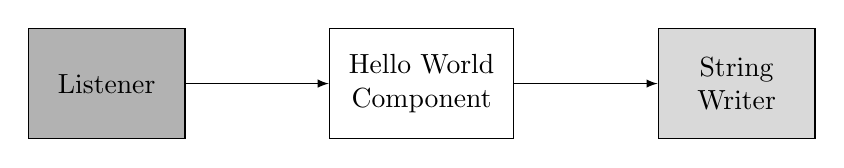
\begin{tikzpicture}[node distance = 2cm, auto]
    % Nodes
    \node [listener] (listener) {Listener};
    \node [component, right of=listener, text width=6em,, node distance=4cm] (hello) {Hello World Component};
    \node [writer, right of=hello, node distance=4cm] (writer) {String Writer};
    % Edges
    \path [line] (listener) -- (hello);
    \path [line] (hello) -- (writer);
\end{tikzpicture}
\caption[scale=1.0]{Hello world! server architecture.}
\label{fig:helloWorld}
\end{figure}

The \texttt{Listener} represents the 
part of the program that gets requests and feeds them to the network.
The \texttt{Hello World Component} inputs a client request from its input channel
and outputs the request together with the Hello World! string that should be 
used as a response to its output channel.
The \texttt{String Writer} writes the text response back to the client.

This is a good example of the basic components of the suggested framework.
We can call the three main parts the \texttt{Listener}, \texttt{Processor} 
and \texttt{Writer}, where
the \texttt{Listener} catches the incoming requests and feeds them into the network,
the \texttt{Processor} processes them and the \texttt{Writer} writes the generated result 
back to the client. That is \texttt{Listener} is the start and \texttt{Writer}
is the end of the server pipeline.

\subsection{File Server}
\label{sec:fileServer}
Architecture of a simple file server follows the architecture of the Hello world!
server introduced above. It consists of a \texttt{Listener}, which catches the requests,
\texttt{File Getter}, what is a function that gets the requested file (that is it
constructs the absolute path to the requested file and loads it into the memory) 
and finally there is a \texttt{File Writer}, which
writes the file to the client. The architecture is shown in Figure \ref{fig:fileServer}.
\begin{figure}[h]
\centering
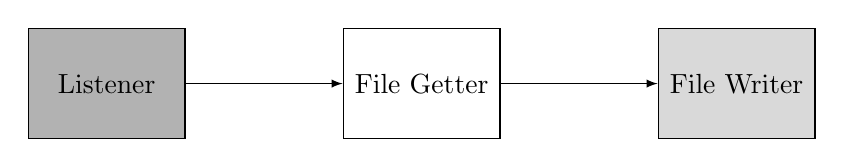
\begin{tikzpicture}[node distance = 2cm, auto]
    % Nodes
    \node [listener] (listener) {Listener};
    \node [component, right of=listener, node distance=4cm] (getter) {File Getter};
    \node [writer, right of=getter, node distance=4cm] (writer) {File Writer};
    % Edges
    \path [line] (listener) -- (getter);
    \path [line] (getter) -- (writer);
\end{tikzpicture}
\caption[scale=1.0]{File server.}
\label{fig:fileServer}
\end{figure}

If we want to compress some subset of files, we can just add a \texttt{Splitter}
that sends files that are supposed to be compressed to a \texttt{Gzip Writer}, which
compresses the file and writes the result to the client. The rest of the files
will be passed to the standard \texttt{File Writer}. This architecture is shown in
Figure \ref{fig:fileServer2}.

\begin{figure}[h]
\centering
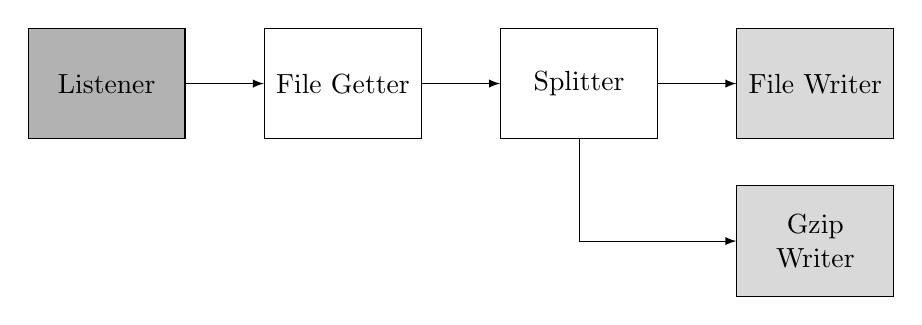
\begin{tikzpicture}[node distance = 2cm, auto]
    % Nodes
    \node [listener] (listener) {Listener};
    \node [component, right of=listener, node distance=3cm] (getter) {File Getter};
    \node [component, right of=getter, node distance=3cm] (splitter) {Splitter};
    \node [writer, right of=splitter, node distance=3cm] (fwriter) {File Writer};
    \node [writer, below of=fwriter] (gwriter) {Gzip Writer};
    % Edges
    \path [line] (listener) -- (getter);
    \path [line] (getter) -- (splitter);
    \path [line] (splitter) -- (fwriter);
    \path [line] (splitter) |- (gwriter);
\end{tikzpicture}
\caption[scale=1.0]{File server with compression.}
\label{fig:fileServer2}
\end{figure}

\subsection{Caching}
Suppose we have a worker component, which performs some expensive computation
and that we want to cache its output.
Using the proposed architecture we can just wrap the worker in a caching layer.
That is we only run the worker component if we don't have the result
in the cache, otherwise we just return the stored result. 
This design is show in Figure \ref{fig:caching}.

\begin{figure}[h]
\centering
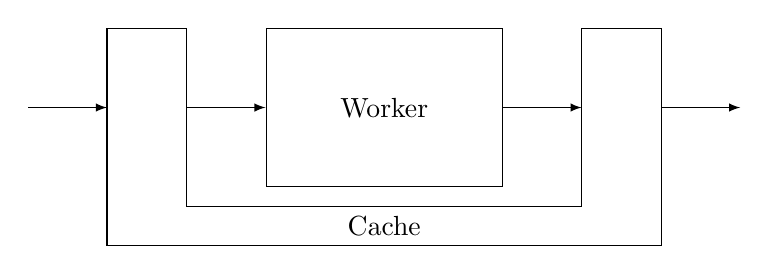
\begin{tikzpicture}[
    workerWidth/.style={minimum width=3cm},
    workerHeight/.style={minimum height=2cm},
    UWidth/.style={minimum width=1cm},
    every node/.style={
        text centered,
        }
        ]
    \node[workerWidth, workerHeight, draw] (worker) at (0, 0) {Worker};

    \node[anchor=north, workerWidth, yshift=-0.25cm] (cache) at (worker.south) {Cache};

    \node[anchor=east, workerHeight, UWidth, xshift=-1cm] (left) at (worker.west) {};
    \node[anchor=west, workerHeight, UWidth, xshift=1cm] (right) at (worker.east) {};

    \draw (left.north west) -- (left.west |- cache.south) -- (right.east |- cache.south) -- (right.north east) -- (right.north west) -- (right.west |- cache.north) -- (left.east |- cache.north) -- (left.north east) -- cycle;

    \draw[<-, >={latex}] (left.west) -- ++(-1, 0);
    \draw[->, >={latex}] (left.east) -- (worker.west);
    \draw[->, >={latex}] (worker.east) -- (right.west);
    \draw[->, >={latex}] (right.east) -- ++(1, 0);
\end{tikzpicture}\caption[scale=1.0]{Caching output of a worker component.}
\label{fig:caching}
\end{figure}

\subsection{Load Balancing}
If there is a lot of traffic in a certain part of the network we can
increase the throughput there
by creating multiple instances of the components in this part of 
the pipeline. The incoming request can then be passed to the component that is 
ready first. When the load in a given part of the pipeline decreases,
we can shut down the created components.

The benefit of the proposed architecture is that, we can do these adjustments
in runtime.
That is, based on current number of requests going through a certain part of 
the network we can decide to add or remove parts of the pipeline. This does not
have to be only adding components locally.
If we use channels over network then
we can connect to other servers and distribute the workload among them.
Hence we can start or shut down other servers based on the current traffic.
See Figure \ref{fig:loadBalancing}.

\begin{figure}[h]
\centering
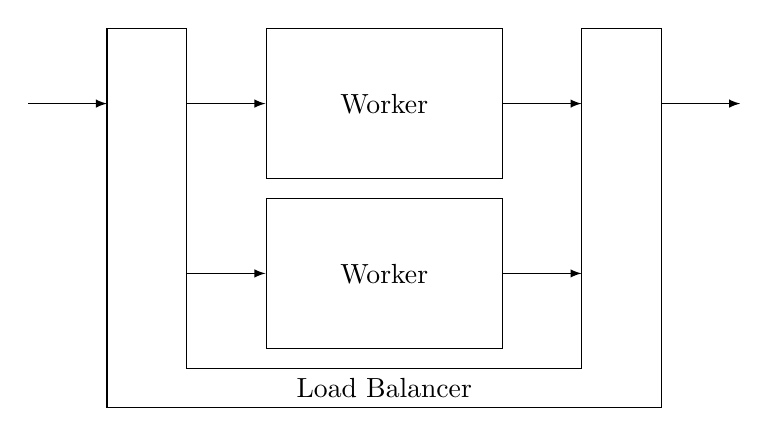
\begin{tikzpicture}[
    workerWidth/.style={minimum width=3cm},
    workerHeight/.style={minimum height=1.9cm},
    UWidth/.style={minimum width=1cm},
    every node/.style={
        text centered,
        }
        ]
    \node[workerWidth, workerHeight, draw] (worker) at (0, 0) {Worker};
    \node[workerWidth, workerHeight, yshift=-1.2cm, draw] (worker2) at (worker.south) {Worker};

    \node[anchor=north, workerWidth, yshift=-0.25cm] (cache) at (worker2.south) {Load Balancer};

    \node[anchor=east, workerHeight, UWidth, xshift=-1cm] (left) at (worker.west) {};
    \node[anchor=west, workerHeight, UWidth, xshift=1cm] (right) at (worker.east) {};
    \node[anchor=east, workerHeight, UWidth, xshift=-1cm] (left2) at (worker2.west) {};
    \node[anchor=west, workerHeight, UWidth, xshift=1cm] (right2) at (worker2.east) {};

    \draw (left.north west) -- (left.west |- cache.south) -- (right.east |- cache.south) -- (right.north east) -- (right.north west) -- (right.west |- cache.north) -- (left.east |- cache.north) -- (left.north east) -- cycle;

    \draw[<-, >={latex}] (left.west) -- ++(-1, 0);
    \draw[->, >={latex}] (left.east) -- (worker.west);
    \draw[->, >={latex}] (worker.east) -- (right.west);
    \draw[->, >={latex}] (left2.east) -- (worker2.west);
    \draw[->, >={latex}] (worker2.east) -- (right2.west);
    \draw[->, >={latex}] (right.east) -- ++(1, 0);
\end{tikzpicture}\caption[scale=1.0]{
    Managing load in a given part of the network.
    One of the workers can be shut down or more workers can be added.
}
\label{fig:loadBalancing}
\end{figure}

\subsection{Comparison to Apache server configuration}

\subsection{Summary}

%%%%%%%%%%%%%%%%%%%%%%%%%%%%%%%%%%%%%%%%%%%%%%%%%%%%%%%%%%%%%%%%%%%%%%%
%%%%%%%%%%%%%%%%%%%%%%%%%% Implementation %%%%%%%%%%%%%%%%%%%%%%%%%%%%%
%%%%%%%%%%%%%%%%%%%%%%%%%%%%%%%%%%%%%%%%%%%%%%%%%%%%%%%%%%%%%%%%%%%%%%%

\newpage
\section{Implementation}
\label{sec:impl}
In this Chapter I present basic elements of my \texttt{mpserver} toolkit
and how to work with them. The most important are the primitive types:
\texttt{Value}, \texttt{Component} and \texttt{Writer}.

\subsection{Values}
\texttt{Value} is a struct type that represents the type of messages that are
passed between the components of the network. It is defined as follows:

\begin{figure}[h]
\centering
\begin{lstlisting}
type Value struct {
    Request *http.Request
    Writer http.ResponseWriter
    Result Any
    Done chan<- bool
    ResponseCode int
}
\end{lstlisting}
\caption[scale=1.0]{Declaration of type Value.}
\label{fig:Value}
\end{figure}

Here:
\begin{itemize}
  \item \texttt{Request} is the HTTP request made by the client implemented
        in the default HTTP library.

  \item \texttt{Writer} is an object that writes the response back to the client.
        This field should only be used by \texttt{Writer} objects that are introduced later.
        Its type is \texttt{ResponseWriter}, which is implemented in the default HTTP
        package. This field together with the \texttt{Request} field is set just before
        the value is fed into the network.

  \item \texttt{Result} is the result computed so far (initially nil). This is
        of type \texttt{Any} which is defined to be the empty interface.
        This allows values of any type to be stored there.

  \item \texttt{Done} is a signaling channel. Signal should be send on this channel,
		after the response is written at the end of the pipeline. This
        allows the connection to the client to be closed after the result
        is written.

  \item \texttt{ResponseCode} is the HTTP response code that should be 
        returned to the client. The default value of this field is 200,
        which represents a successful request.
\end{itemize}


\subsection{Components}
This section introduces the component type, then shows how we can simply
create components and finally presents a way how multiple components can
be combined to form a liner pipeline.

\subsubsection{The Component type}
Component is a generic part of the pipeline with an input and output channel.
It processes the values provided on input channel and outputs the results
on the output channel. The type \texttt{Component} is defined as follows:
\begin{lstlisting}
type Component func (in <-chan Value, out chan<- Value)
\end{lstlisting}
Every component should satisfy the following conditions:
\begin{itemize}
    \item When run a component should eventually read all values that are
          written to its input channel.

    \item Every value that a component reads from its input channel
          should be written to its output channel after the value was processed
          and possibly modified. This ensures that every request gets a response.

    \item A component can terminate only when its input channel is closed 
          Before terminating, the component should close its output channel.
          This ensures termination of any components further down in the network.

    \item Component can only close its output channel and it can only do so
    	  after its input channel have been closed. It shouldn't attempt
          to close the input channel as this will likely result in an exception.
\end{itemize}

\subsubsection{Making Components}
To simplify the construction of components, so that they adhere to 
the above specification the package provides a helper function that 
constructs a component using a function that maps one \texttt{Value} object 
into another \texttt{Value} object. 
That is the function has the following signature:
\begin{lstlisting}
type ComponentFunc func (val Value) Value
\end{lstlisting}
This represents the mapping of the input values to the output values. 

Now the code for the described component generator is below:
\begin{figure}[h]
\centering
\begin{lstlisting}
func MakeComponent(f ComponentFunc) Component {
    return func (in <-chan Value, out chan<- Value) {
        for val := range in {
            out <- f(val)
        }
        close(out)
    }
}
\end{lstlisting}
\caption[scale=1.0]{Declaration of MakeComponent function.}
\label{fig:MakeComponent}
\end{figure}

Here the for loop reads values from the input channel and assigns them
to the variable \texttt{val} while the input channel is open. Then the 
the function \texttt{f} is applied to this value and the result is outputted.
Afterwards, the component waits for another value. When the input channel
is closed the loop terminates. Afterwards, the component closes its output channel
and terminates.

\subsubsection{Constant Component}
Constant Component is a simple component generator that takes a value c
of any type and returns a component that writes c to the Result field of 
all inputted values and then outputs them. It's definition using the 
\texttt{MakeComponent} generator is show below.
\begin{lstlisting}
func ConstantComponent(c Any) Component {
    return MakeComponent(func (val Value) Value {
        val.Result = c; return val
    })
}
\end{lstlisting}

\subsubsection{Linking components}
The library also provides a component generator \texttt{LinkComponents} that takes 
any number of components and returns a component that behaves as their 
linear combination. That is as a pipeline constructed from these components 
in the order in which they are provided. Its signature is shown below.
\begin{lstlisting}
func LinkComponents(components ...Component) Component
\end{lstlisting}
The subcomponents are linked and run when the combined component is run. 
The last of the provided components is run in the goroutine in which
the combined component was run.

\subsection{Writers}
Here, I introduce the \texttt{Writer} type, which acts as the end of the 
pipeline. Then I present a special writer for writing errors and a way
of separating error values from the stream of all values.
\subsection{Writer type}
Writer is the end of the pipeline which writes results to the client.
The type \texttt{Writer} is defined as follows:
\begin{lstlisting}
type Writer func (in <-chan Value, errChan chan<- Value)
\end{lstlisting}
It is a function with an input channel and a channel for reporting errors.
Every writer should satisfy the following:
\begin{itemize}
	\item Once a writer writes the result to the client, it should send a signal
		  on the Done channel, so that the connection to the client can be closed.
	\item The writer terminates when its input channel is closed. It shouldn't
		  close the error channel, as other processes might be using it.
\end{itemize}
The package provides writers to write string, json and file responses
using multiple input types.

\subsubsection{Error Writer}
Error Writer is a function that writes error responses to the client.
It has the following signature:
\begin{lstlisting}
func ErrorWriter(in <-chan Value)
\end{lstlisting}
It has only one input channel. The writer terminates when the channel
is closed. The channel should be closed only after all Writers that 
are using it terminated.

Note that this is a special writer as it doesn't match the \texttt{Writer} type. 
It collects the error responses from all other writers and all other parts
of the network. It also logs all the responses on the standard input for
purposes of debugging.

\subsubsection{Error Splitter}
If we allow error messages to reach any other writer than the error writer,
all errors will only show that a particular writer got a wrong input.
To avoid this the package provides \texttt{ErrorSplitter} function, which
has the signature shown below.
\begin{lstlisting}
func ErrorSplitter(in <-chan Value, out chan<- Value, 
                                    errChan chan<- Value)
\end{lstlisting}
This function sends all values with an error in the Result field to the 
error channel, which should lead to the error writer. All other result 
are send to the output channel. Hence, this acts as error separator.
It is usually used just before a normal response writer.

\subsection{Conditions and Splitter}
In this section I introduce a way to split a stream of incoming values into
multiple streams of values that go into different parts of the network
using very flexible rules for splitting.

\subsubsection{Conditions}
Condition type is defined as follows:
\begin{lstlisting}
type Condition func (val Value) bool
\end{lstlisting}
It is a just function that takes a value and returns a boolean.

\subsubsection{Splitter}
Conditions are used in Splitter, which is a component with the 
following signature:
\begin{lstlisting}
func Splitter(in <-chan Value, defOut chan<- Value, 
			  outs []chan<- Value, conds []Condition)
\end{lstlisting}
It takes an input channel, default output channel, array of output channels and array of conditions.
The number of output channels and the number of conditions should be the same.
For every input value the Splitter evaluates the conditions from first to last.
When a condition returns true the value is written to a corresponding output channel 
and the processing of the current value terminates. If all conditions return false
then the value is written to the default output channel.

\subsection{Summary}
In this Chapter I introduced the basic elements of the library. This 
is enough to implement some simple serves. The next section introduces
more advanced components that allow more complex behaviors.

%%%%%%%%%%%%%%%%%%%%%%%%%%%%%%%%%%%%%%%%%%%%%%%%%%%%%%%%%%%%%%%%%%%%%%%
%%%%%%%%%%%%%%%%%%%%%%%%%% Implementation 2 %%%%%%%%%%%%%%%%%%%%%%%%%%%
%%%%%%%%%%%%%%%%%%%%%%%%%%%%%%%%%%%%%%%%%%%%%%%%%%%%%%%%%%%%%%%%%%%%%%%

\newpage
\section{Advanced component generators}
\label{sec:impl2}
In this section I introduce more advanced component generators for caching,
session management, load balancing, network communication and error handling.

\subsection{Storage}
Storage is an interface representing thread safe mapping from string keys
to values of any type. Its definition is shown below.
\begin{lstlisting}
type Storage interface {
    Get(string) (interface{}, bool)
    Set(string, interface{})
    Remove(string)
    CompareAndRemove(string, interface{}) bool
    Keys() []string
}
\end{lstlisting}
The package provides a default implementation of this interface that
stores the data in memory using (with minor modifications) sharded concurrent map implementation
by Or Hiltch\footnote{Code available at \url{https://github.com/orcaman/concurrent-map}}.
If a developer wants to store the values in the 
database instead, they can provide their own implementation of the store interface
and use any component that uses the storage the same way as before.
This makes the components that use the storage highly configurable.


\subsection{States and Session Management Component}
\subsubsection{States}
State is an interface defined as follows:
\begin{figure}[h]
\centering
\begin{lstlisting}
type State interface {
    Next(val Value) (State, error)
    Terminal() bool
    Result() Any
}
\end{lstlisting}
\caption[scale=1.0]{Declaration of the State interface.}
\label{fig:State}
\end{figure}

Here the expected behavior of the member functions is as follows:
\begin{itemize}
	\item The \texttt{Next} function returns the next state when provided with a value.
	\item The \texttt{Terminal} function indicates whether the current state is a terminal state.
	\item The \texttt{Result} function returns the result that possibly after further 
		  processing should be returned to the client.
\end{itemize}

\subsubsection{Session Management Component}
\texttt{SessionManagementComponent} is a following component generator.
\begin{lstlisting}
func SessionManagementComponent(store Storage, initial State, 
                seshExp time.Duration, useCleaner bool) Component
\end{lstlisting}

It arguments are a storage object to be used, an initial state for each session,
a session expiration time and a boolean indicating whether expired
entries should be automatically removed from the map.
The returned component behaves as a session manager. 
It behaves as follows:

The component stores a mapping from session ids to current state of the session.

Every new request gets assigned a unique session id. Then a mapping from the generated 
id to the current state, which is generated from the initial state using the provided value,
is stored. The result of the call to the \texttt{Result} function on the next state with the provided 
value is then sent down the pipeline.

When a request with set `Session-Id` header comes in, the component gets the current 
state for the session and gets the next state for it based on the provided value.
The mapping is then updated with the generated state and the result from the current state
is passed down the pipeline.

When a session reaches a Terminal state, the session id is removed from the map
and the final result is outputted.

The states in the mapping are timestamped and are removed from the map after
the session expiration time, if they haven't finished before that.

% More hype
The abstraction using states allows the users of the package to implement the
logic for the session, independently of the session management part.

\subsection{Caching}
\texttt{CacheComponent} is a Component generator with the following signature:
\begin{figure}[h]
\centering
\begin{lstlisting}
func CacheComponent(cache Storage, worker Component, 
            expiration time.Duration, useCleaner bool) Component
\end{lstlisting}
\caption[scale=1.0]{Type signature of the \texttt{Cache Component} generator.}
\label{fig:cacheComp}
\end{figure}

The returned component behaves as follows:
\begin{itemize}
	\item When a value is input that the component hasn't seen before, then
		  the value is passed to the provided worker and the result is stored in
		  a map.
	\item When the component gets a previously seen value, it returns the value
		  stored in the map, if it hasn't expired yet. If it expired, then the component
		  treats it as a new value.
	\item Expired values are regularly deleted from the map if the useCleaner
          option is set to \texttt{true}.
\end{itemize}

For the generated component to function properly, the worker must output
a value for every value that is sent to it. This is one of the conditions
that a component must meet, so this shouldn't be an issue.

\subsection{Load Balancing}
\texttt{LoadBalancingComponent} is a Component generator with the following signature:
\begin{figure}[h]
\centering
\begin{lstlisting}
func LoadBalancingComponent(addTimeout, 
		removeTimeout time.Duration, worker Component) Component
\end{lstlisting}
\caption[scale=1.0]{Declaration of Load Balancing Component generator.}
\label{fig:loadComp}
\end{figure}
The returned component has an array of workers which can be easily shut down.
The initial number of workers is 1. 

For every input value, the component behaves as follows:
\begin{itemize}
	\item It tries to send the value to the workers, if this is not successful, 
		  before the \texttt{addTimeout}, then the component creates a new worker and then
		  tries to send the value to the workers again. This will be successful because
		  there is at least one worker that is not busy.
	\item The workers send their results further down the pipeline.
	\item If there are no incoming values for duration equal to the \texttt{removeTimeout},
          then the component shuts down one of the workers, if there is more than one worker.
	\item When the input channel of the component is closed, then the load balancer shuts down all
		  the workers, then it closes its output channel and terminates.
\end{itemize}
There are a lot of other possible load balancing strategies. 
Implementing them should be a simple modification of the existing code.
Note that this is very powerful concept as it can also be used to share
the load between multiple servers (here using a different strategy might be 
preferred).

\subsection{Error handling}
% TODO: maybe add a diagram
\subsubsection{Error Passer}
As a lot of components expect an input of a certain type, their execution
might end with an error if they are provided with an error result from
a previous component. This would make debugging very hard. Hence, the 
package provides the following component wrapper, that won't pass errors
to the provided component. This signature of this wrapper is shown below.
\begin{figure}[h]
\centering
\begin{lstlisting}
func ErrorPasser(worker Component) Component
\end{lstlisting}
\caption[scale=1.0]{Declaration of Error Passer Component generator.}
\label{fig:ErrorPasser}
\end{figure}

The generated component behaves as follows:
\begin{itemize}
	\item For every input value it checks whether the result is an error
		  and if that is the cases it just outputs the value.
	\item If the result of the input value is not an error, then the component
		  passes the value to the worker, which after processing it passes 
		  it further down the pipeline.
\end{itemize}

\subsubsection{Panic handling component}
If we use a component which might cause panic, this will crash the whole
server when the panic occurs. Hence, the package provides the 
\texttt{PanicHandlingComponent}. The signature of this wrapper is shown 
below.
\begin{figure}[h]
\centering
\begin{lstlisting}
func PanicHandlingComponent(worker Component) Component
\end{lstlisting}
\caption[scale=1.0]{Declaration of Panic Handling Component generator.}
\label{fig:panicHandler}
\end{figure}

It takes a component that can cause panic and returns a component the 
behaves as follows:
\begin{itemize}
	\item It passes every input value to the worker, gets the result 
          from it and then passes the result further down the pipeline.
	\item In case the worker crashes, that is causes panic, the component 
          writes an error as a result for the value that caused the crash 
          and the restarts the worker.
	\item The component can itself cause a panic if the worker closes its 
          input channel, or if it closes its output channel before its input 
          channel is closed. That is if the worker violates the contract
          for components.
\end{itemize}

\subsection{Network Components}
In this section I present a component generator that can make network
requests. Then I introduce a helper component that alters incoming 
requests, so that they can be performed again using a different host
and a component that processes HTTP responses. Finally, I show how
can these components be plugged together to act as a proxy server. 

\subsubsection{Network Component}
Network Component is a component generator with the following signature:
\begin{figure}[h]
\centering
\begin{lstlisting}
func NetworkComponent(client *http.Client) Component
\end{lstlisting}
\caption[scale=1.0]{Declaration of Network Component generator.}
\label{fig:NetworkComponent}
\end{figure}

It takes a single parameter, which is an http client.
The generated component for each input value makes an http request,
taken from the Result field of the value, using the provided http client.
If there is no request in the Result field or the request fails, then
the component returns an appropriate error. 

Note that the result of the request is fetched in the goroutine where the
component runs. Hence, slow requests might block the pipeline. To avoid
this behavior the \texttt{NetworkComponent} is usually used together with one
of the load managers.

\subsubsection{Request Copier}
Request Copier is a component generator with the following signature:
\begin{figure}[h]
\centering
\begin{lstlisting}
func RequestCopier(scheme, host string) Component
\end{lstlisting}
\caption[scale=1.0]{Declaration of Request Copier Component generator.}
\label{fig:RequestCopier}
\end{figure}
It takes string parameters scheme (e.g. http) and host (e.g. www.google.com) 
and returns a component that for each input value copies the Request made 
by the client to the Result field and updates it with the given scheme and 
path and then outputs this value.

\subsubsection{Response Processor}
The \texttt{Response} type of the mpserver package is defined as a following struct:

\begin{figure}[h]
\centering
\begin{lstlisting}
type Response struct {
		Header http.Header
		Body []byte
}
\end{lstlisting}
\caption[scale=1.0]{Declaration of type Response.}
\label{fig:Response}
\end{figure}

It holds the header and body of a http response. The difference between
this definition and the definition in the default http package is that
the body of my response is a slice of bytes. That is the body have already been
read and the connection to server has been closed.

The Response Processor is a component that for each input value
looks if provided Result is the default http Response, and if it is
it then reads it and transfers it to mpsever Response type, which it
then writes to the Result field and outputs the value. If no response
is provided, then the component outputs an appropriate error.

To use this component after the Network component, the Response Processor
should be wrapped in an error passing component, so that when the 
Network component fails, then the response processor won't have to do
any work.

\subsubsection{Proxy Component}
Proxy component is a combination of Request Copier, Network component 
and Response processor in a linear pipeline. It acts as a proxy server
in the following sense. It forwards the provided request to the specified
host and then reads and outputs the response. 

All components are wrapped
in an Error passer to avoid doing unnecessary work and to make the component
more robust. Its implementation is shown below:

\begin{figure}[h]
\centering
\begin{lstlisting}
func ProxyComponent(scheme, host string, 
					client *http.Client) Component {
	return LinkComponents(
		ErrorPasser(RequestCopier(scheme, host)),
		ErrorPasser(NetworkComponent(client)),
		ErrorPasser(ResponseProcessor))
}
\end{lstlisting}
\caption[scale=1.0]{Declaration of Proxy Component generator.}
\label{fig:ProxyComp}
\end{figure}

\subsection{Summary}
In this section I introduced more advanced component wrappers and generators
and described a way to use them. The next section shows a few example
servers implemented using my toolkit.

%%%%%%%%%%%%%%%%%%%%%%%%%%%%%%%%%%%%%%%%%%%%%%%%%%%%%%%%%%%%%%%%%%%%%%%
%%%%%%%%%%%%%%%%%%%%%%%%%%%%%% Examples %%%%%%%%%%%%%%%%%%%%%%%%%%%%%%%
%%%%%%%%%%%%%%%%%%%%%%%%%%%%%%%%%%%%%%%%%%%%%%%%%%%%%%%%%%%%%%%%%%%%%%%

\newpage
\section{Examples}
\label{sec:examples}
\subsection{Hello world! server}
Figure \ref{fig:HelloWorldImpl} shows the Implementation of the Hello World!
server described in section \ref{sec:helloWorld}.
It's a direct translation of the diagram shown in Figure \ref{fig:helloWorld}.

The Listener corresponds to the call of mpserver.Listen function.
Hello world Component translates into an instance of ConstantComponent
and String Writer is the writer in the package with the same name.
We plug these together using two channels, start the components 
and then start the server itself.

\begin{figure}[h]
\centering
\begin{lstlisting}
package main

import(
    "log"
    "net/http"
    "mpserver"
)

func main() {
    in := mpserver.GetChan()
    out := mpserver.GetChan()

    mux := http.NewServeMux()
    mpserver.Listen(mux, "/hello", in)

    go mpserver.ConstantComponent("Hello world!")(in, out)
    go mpserver.StringWriter(out, nil)
    
    log.Println("Listening on port 3000...")
    http.ListenAndServe(":3000", mux)
}
\end{lstlisting}
\caption[scale=1.0]{Implementation of the Hello World! server.}
\label{fig:HelloWorldImpl}
\end{figure}

\newpage
\subsection{File server}
Figure \ref{fig:FileServerImpl} shows the implementation of a simple 
file server that compresses all '.go' files. It is almost a direct translation
of the diagram shown in figure \ref{fig:fileServer2} in section \ref{sec:fileServer}.
However, here the File Getter is composed of two parts, which are \texttt{PathMaker}
and \texttt{FileComponent}. The \texttt{PathMaker} firstly strips a given
prefix from the request path and then prepends a provided directory name to 
the result. The \texttt{FileComponent} tries to open a file at a path 
provided in the result field of the incoming value. Other modifications
are the addition of the \texttt{ErrorWriter} and the channel going to it from
the \texttt{Splitter}.
This path is used when a non existent file is requested be the client.
Otherwise '.go' files goes to the \texttt{GzipWriter} and all other files to 
the standard \texttt{FileWriter}.
The diagram that represents this server is shown in 
Figure \ref{fig:fileServer3}.

\begin{figure}[h]
\centering
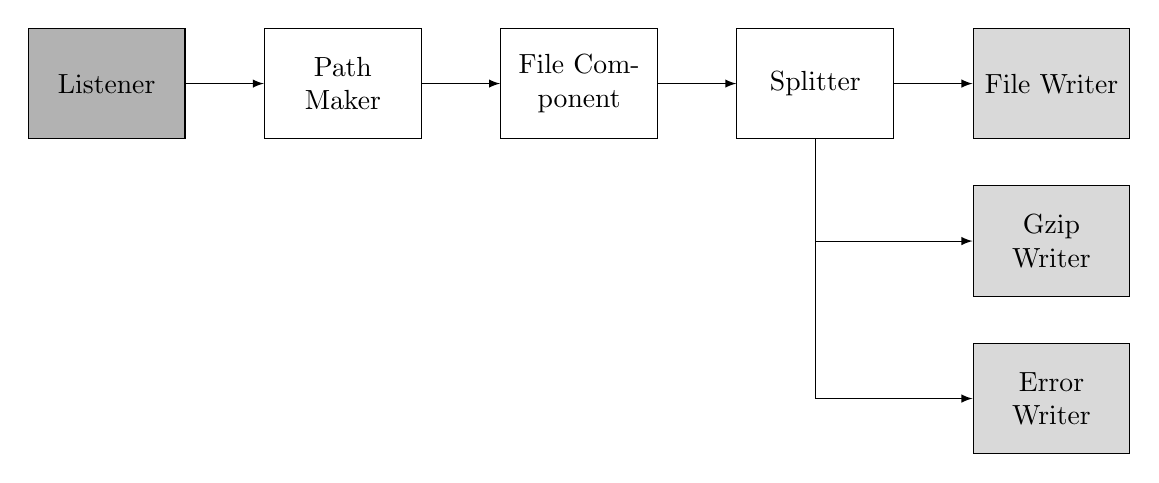
\begin{tikzpicture}[node distance = 2cm, auto]
    % Nodes
    \node [listener] (listener) {Listener};
    \node [component, right of=listener, node distance=3cm] (maker) {Path Maker};
    \node [component, right of=maker, node distance=3cm] (comp) {File Component};
    \node [component, right of=comp, node distance=3cm] (splitter) {Splitter};
    \node [writer, right of=splitter, node distance=3cm] (fwriter) {File Writer};
    \node [writer, below of=fwriter] (gwriter) {Gzip Writer};
     \node [writer, below of=gwriter] (ewriter) {Error Writer};
    % Edges
    \path [line] (listener) -- (maker);
    \path [line] (maker) -- (comp);
    \path [line] (comp) -- (splitter);
    \path [line] (splitter) -- (fwriter);
    \path [line] (splitter) |- (gwriter);
    \path [line] (splitter) |- (ewriter);
\end{tikzpicture}
\caption[scale=1.0]{File server with compression and error handling.}
\label{fig:fileServer3}
\end{figure}

\begin{figure}
\begin{lstlisting}
package main
import(
    "log"
    "net/http"
    "mpserver"
    "strings"
)
// Test if the provided value contains an error in the Result
func isError(val mpserver.Value) bool {
    _, isErr := val.Result.(error)
    return isErr
}
// Test if the path of the requested file ends with .go
func isGoFile(val mpserver.Value) bool {
    return strings.HasSuffix(val.Request.URL.Path, ".go")
}

func main() {
    // Construct the channels
    in := mpserver.GetChan()
    toFileComp := mpserver.GetChan()
    toSplitter := mpserver.GetChan()
    compressed := mpserver.GetChan()
    errChan := mpserver.GetChan()
    splitterOut := mpserver.ToOutChans(
        []mpserver.ValueChan{errChan, compressed})
    uncompressed := mpserver.GetChan()

    // Start the file components
    go mpserver.PathMaker("files", "")(in, toFileComp)
    go mpserver.FileComponent(toFileComp, toSplitter)
    
    // Start the splitter
    go mpserver.Splitter(toSplitter, uncompressed, splitterOut, 
                         []mpserver.Condition{isError, isGoFile})

    // Start the writers
    go mpserver.GzipWriter(compressed, errChan)
    go mpserver.GenericWriter(uncompressed, errChan)
    go mpserver.ErrorWriter(errChan)

    // Start the server
    mux := http.NewServeMux()
    mpserver.Listen(mux, "/", in)
    log.Println("Listening on port 3000...")
    http.ListenAndServe(":3000", mux)
}
\end{lstlisting}
\caption[scale=1.0]{Implementation of a File Server that compresses go files.}
\label{fig:FileServerImpl}
\end{figure}

\subsection{Proxy server}
a

%%%%%%%%%%%%%%%%%%%%%%%%%%%%%% Shopping %%%%%%%%%%%%%%%%%%%%%%%%%%%%%%%
\newpage
\section{Building a shopping server}
\label{sec:shopping}

%%%%%%%%%%%%%%%%%%%%%%%%%%%%%% Testing %%%%%%%%%%%%%%%%%%%%%%%%%%%%%%%%
\newpage
\section{Performance Testing}
\label{sec:test}
%%%%%%%%%%%%%%%%%%%%%%%%%%%%% Conclusion %%%%%%%%%%%%%%%%%%%%%%%%%%%%%%
\newpage
\section{Conclusion}
\label{sec:conclusion}

\subsection{Related work}
Similar work has been done by James Whitehead II in \cite{whitehead}.
However, his approach is rather different than the approach used 
in this project. He uses reader-writer pairs for communication between
two different components in the network. This requires to construct the
reader and writer objects for each pair of communicating components
for all requests.
In order to construct these readers and writers a connection object is 
passed through the network.
I believe this indirect approach introduces unnecessary overhead and 
makes it more difficult to understand how the toolkit works.

%%%%%%%%%%%%%%%%%%%%%%%%%%%% Bibliography %%%%%%%%%%%%%%%%%%%%%%%%%%%%%
\newpage
\printbibliography[
    heading=bibintoc,
    title={References}
]

\end{document}




